\chapter{Clustering on Graphs}

Clustering is a procedure applied to datasets where the output is groupings of the datapoints such that each group, referred to as cluster, shares some kind of similarity within groups. The definition is not precise because clustering can span the spectrum between supervised (eg. community detection with ground truth) and unsupervised problems (eg. data exploration).  Naturally, the technique can be data driven or model driven.  In the former we let the  features in datasets motivate definitions of similarity metrics and even suggest ground truth.  In the latter, a probabilistic generative model is often used, where the generative mechanism defines the ground truth communities.  The two approaches are not unrelated.  Generative models, for instance, are designed to mimic statistics of real graphs.  The Stochastic Blockmodel is an example of such a benchmark artificial dataset and we will discuss it in detail.  


\begin{figure}[h]
\begin{center}
  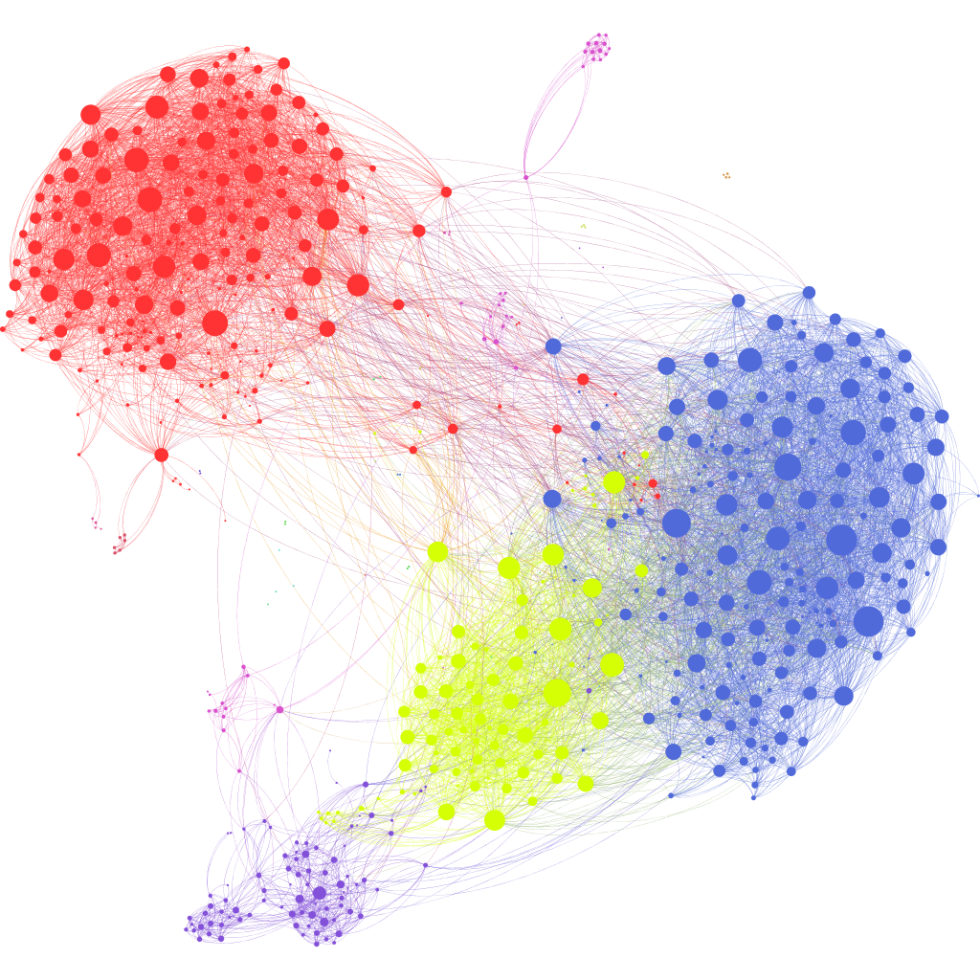
\includegraphics[scale=0.15]{social_network.png}
  \caption{A sampling of a Facebook friend network.\cite{social_network}}
  \label{fig:socialnet}
 \end{center}
\end{figure}

\begin{figure}
\begin{center}
  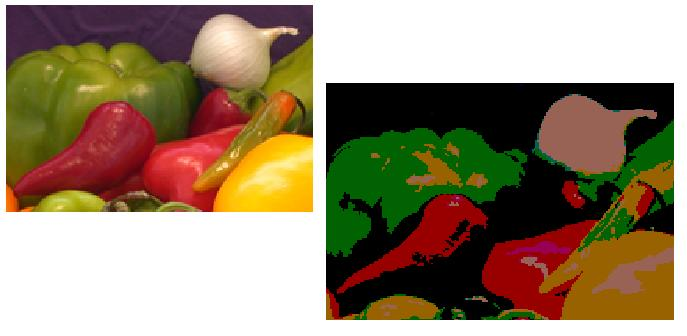
\includegraphics[scale=0.35]{image_segmentation.jpg}
  \caption{A result of image segmentation.\cite{image_seg}}
  \label{fig:seg}
 \end{center}
\end{figure}

\begin{figure}
\begin{center}
  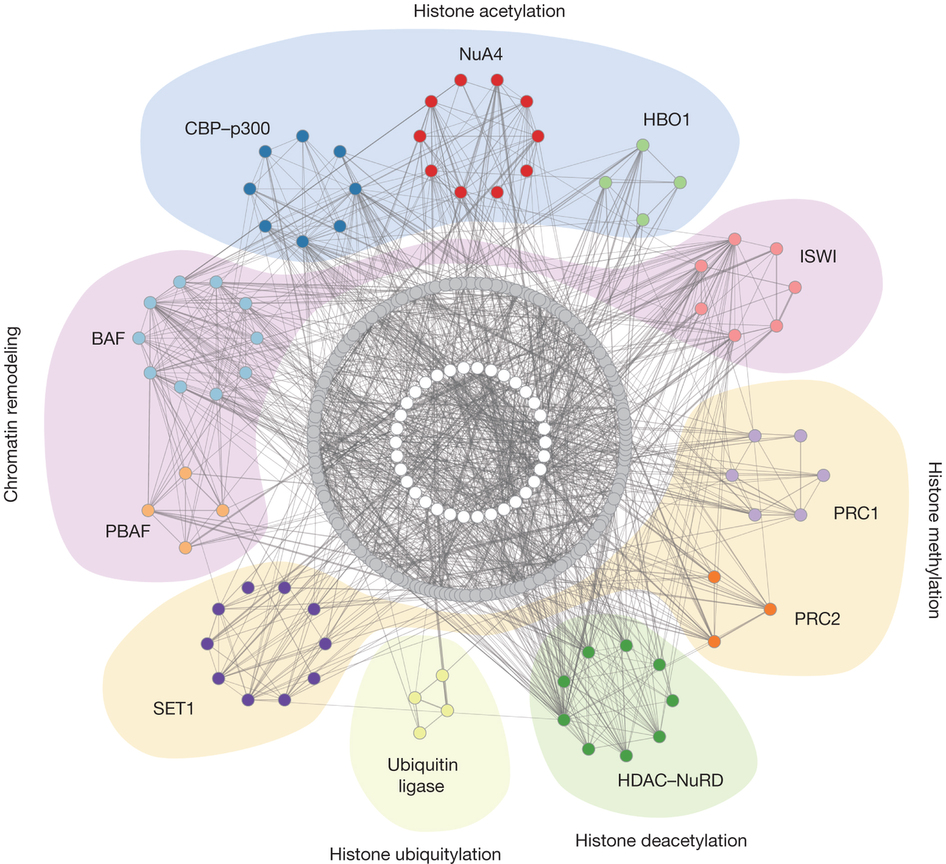
\includegraphics[scale=0.20]{protien_network.jpg}
  \caption{A protein to protein interaction network.\cite{protein}}
  \label{fig:protien}
 \end{center}
\end{figure}

Finding clusters is an important task in many disciplines. Whether to uncover hidden functional similarities in protein interaction networks, or compress data, or improve ecommerce recommendations.  Graph clustering is the clustering procedure applied to a dataset that has graph structure. The goal here is to use the extra topological information of the network to inform clustering choices and similarity measures. Applied to social networks, clustering is oftentimes referred to as community detection. 

We can frame the task of clustering as an inverse problem on graphs.  The goal broadly, is to infer global properties from local interactions.  This second part of the thesis studies how we can use neural networks to do clustering on graphs.  At the root of this task, we aim to make a neural network architecture powerful enough to contain the expressive closure of the state of art algorithms for clustering.  The benefit of the neural network approach is that we do not have to choose what algorithm to use via heuristics or local statistics gathered from the network.  Instead it is data driven.  The model will learn by gradient descent, fitting the best parameters given the distributions of the graphs it learns from.  We will test the model's performance on benchmarked data.  Before discussing the results, we will first go over some preliminaries in both neural networks and the well studied Stochastic Blockmodel.  

